
\chapter{Experimental Results}

\section{Purpose}
The purpose of this experiment is to measure how many insertions, deletion and modifications are performed on the Java AST verses comments across a range of realistic benchmarks. Similarly, how many insert and delete pairs can be classified as moves. 

% establish if there are superficial changes in currently working projects.  
% By superficial we mean that the change does not add much of value apart from 
% personal taste or formatting.  In some cases changes to the order of methods 
% within a class does change the behaviour of a program, this is an example of 
% a superficial change.  It is harder to determine if comments are superficial 
% because certain comments could be important to others and others irrelevant. 
% We will attempt to establish if there are any patterns in comments to 
% determine if they are superficial or not.  Determining if there are 
% superficial change may indicate that there is a separation between personal 
% preferences that would be best contained in a private view and items that 
% need to be shared for collaboration.

\section{Methodology}
We will now outline the experimental methodology. Our goal is make it possible for someone to reproduce our experiment.

The experiment was run on a Lenovo laptop with 3.5GB Ram and 113.2 GB disk space assigned to the 64 bit Ubuntu 13.10 (Saucy Salamander) operating system. The tests were written in Java and run within the Eclipse IDE



 
 
 \begin{table}[H]
    \small{
    \begin{tabular}{l|lllll}
    Benchmark        & Description   & Commits  & LOC   \\ \hline
    Jasm             &  \begin{minipage}[t]{0.5\textwidth}
Java bytecode assembler written for use with the Whiley programming language.

github.com/Whiley/Jasm 
\end{minipage}        & 74      & 29139 \\
    Jpp              & \begin{minipage}[t]{0.5\textwidth}
    Pre-processor for Java based on Bash shell script.
    
github.com/maandree/jpp
\end{minipage}        & 40      & 254   \\
    AST Java         & \begin{minipage}[t]{0.5\textwidth}
    Small parser written to transform Java into an AST.
    
github.com/klangner/ast-java 
\end{minipage}       & 24      & 10174 \\
\begin{minipage}[t]{0.15\textwidth}Java Object Diff\end{minipage} & \begin{minipage}[t]{0.5\textwidth}
Allows two Java objects to be compared at runtime.
     
github.com/SQiShER/java-object-diff 
\end{minipage}        & 291     & 10023 \\
    DiffJ            & \begin{minipage}[t]{0.5\textwidth}
    Diff tool which in addition to ignoring white space ignores changes of ordering in package names for a Java file.
    
github.com/jpace/diffj
\end{minipage}        & 490     & 13712 \\
    IRE              & \begin{minipage}[t]{0.5\textwidth}
    Java library for regular expression matching.
    
github.com/jkff/ire  
\end{minipage}       & 41      & 2714  \\
    Syntax           & \begin{minipage}[t]{0.5\textwidth}
    Compiler compiler used for teaching. 
    
github.com/jaimegarza/syntax 
\end{minipage}        & 89      & 9376  \\

    Auto Refactor           & \begin{minipage}[t]{0.5\textwidth}
    Eclipse plug-in that automatically refactors code 
    
github.com/JnRouvignac/AutoRefactor 
\end{minipage}        & 212      & 13400  \\
    \end{tabular}
    }
\end{table}
 
% 
% The Refactor Categories Tool analyses all the historical changes ever made 
% on a software project by extracting successive revisions from a Git 
% repository using JGit.  Once we have two revisions we need to compare them.  
% To do this we compare each of the Java files in both revisions one by one. 
% We only test the Java file if it has been modified or renamed.  If the file 
% been inserted or deleted we ignore it because there is no way to make a 
% comparison. Once we have established that Java files exist, both in the 
% original and the updated copy, we use the text diff in JGit to compare them. 
% As outlined in section \ref{matchingTextWithAST} we figure out which AST 
% nodes the text changes contain.
% The Refactor Categories Tool splits up the identified blocks of source code 
% into several AST nodes and identifies anything between AST Nodes as being 
% text. @c
This text is further evaluated to determine if it is a change to comments or a change to white space. 
An example of this is if the text comparison detects a single change that inserts two new methods and a comment.  
The Refactor Categories Tool will recognise this as three distinct changes. 
This means that it is possible for the Refactor Categories Tool to notice more changes than a text based comparison. 

We had some garbage collection memory issues with some benchmarks that we were testing. 
To resolve these issues the Refactor Categories Tool was run individually once for each benchmark to further ensure that there were no memory leaks between runs.
We also increased the memory by changing the parameters for the run configuration.  The following parameters were added to the run configuration for the test.

\begin{verbatim}
-Xms512M 
-Xmx4096M
\end{verbatim}



% There are a number of comparison operations that the refactor categories 
% tool investigates
% 
% \begin{description}
% 
%   \item [Delete]
%   <<del>>
%   \item [Insert]
%   <<ins>>
% 
%   \item [Modify]
%   <<mod>>
%   \item [Move]
%   <<mov>>
%   \item [Rename]
%   <<ren>>
%   \item [Equivalent]
%   <<eqv>>
% \end{description}
%  @c
% renames are determined as being something where although the AST label has 
% changed the type of the AST node remains the same and its contents have not 
% been changed in any way.



\section{Results}
\subsection{Overview}
After running the Refactor Categories tool over our benchmark suite we obtained the results shown in Table \ref{tab:results}



\begin{table}[t!]
    \small
    \begin{tabular}{l|llllll|l|lll}
    Benchmark        & \multicolumn{6}{|c|}{Java}           & WS & \multicolumn{3}{|c}{Comments} \\ \cline{2-7} \cline{9-11}
    ~                & Ins  & Del  & Mod  & Mov & Ren & Eqv & ~          & Ins      & Del & Mod  \\ \hline
    Jasm             & 264  & 76   & 385  & 7   & 0   & 0   & 26         & 7        & 6   & 95   \\
    Jpp              & 43   & 9    & 50   & 0   & 0   & 0   & 6          & 1        & 2   & 11   \\
    AST Java         & 87   & 28   & 72   & 1   & 0   & 11  & 5          & 2        & 0   & 22   \\
    \begin{minipage}[t]{0.15\textwidth}Java Object Diff\end{minipage} & 2645 & 1961 & 8862 & 5   & 9   & 183 & 277        & 14       & 39  & 1438 \\
    DiffJ            & 3106 & 3164 & 5192 & 58  & 82  & 18  & 276        & 36       & 39  & 291  \\
    IRE              & 263  & 213  & 640  & 1   & 2   & 30  & 49         & 10       & 3   & 79   \\
    Syntax           & 1142 & 544  & 2216 & 6   & 7   & 12  & 204        & 14       & 81  & 451  \\
    Auto refactor    & 1702 & 1621 & 2809 & 7   & 16  & 25  & 295        & 30       & 16  & 568  \\
    \end{tabular}
    \caption{Results over our benchmark suite showing the number of inserts (INS), deletes (DEL), modifications (MOD), moves (MOV), renames (REN) and equivalences (EQV) for Java AST, comments and white-space (WS) changes}
    \label{tab:results}
\end{table}

The number of text changes that were recognised during text comparison for each benchmark are shown in Table \ref{tab:textcomp}. Note that the values in this table are lower as the Refactor Categories tool detects multiple changes which a text based comparison aggregates.  

\begin{table}[H]
    \centering
    \begin{tabular}{l|lll}
    Benchmark        & \multicolumn{3}{|c}{Text Diff} \\ \hline
    ~                & Ins            & Del & Mod  \\ \hline
    Jasm             & 91             & 44  & 337  \\
    Jpp              & 23             & 3   & 41   \\
    AST Java         & 44             & 15  & 85   \\
    Java Object Diff & 1186           & 837 & 8219 \\
    DiffJ            & 746            & 991 & 3544 \\
    IRE              & 112            & 49  & 465  \\
    Syntax           & 691            & 214 & 1863 \\
    Auto Refactor    & 639            & 309 & 1621 \\
    \end{tabular}
    \caption{The result of doing an ordinary text comparison showing the number of inserts (INS), deletes (DEL) and modifications (MOD)}
    \label{tab:textcomp}
\end{table}



\subsection{Discussion}
Figure \ref{fig:textDifference} show the average for all the benchmarks of the types of operations found during an ordinary text comparison.  
The most common merge operation is when items have been modified.  
This occured on average  almost 73 percent of the time.

\begin{figure}[!t]
 \begin{center}
 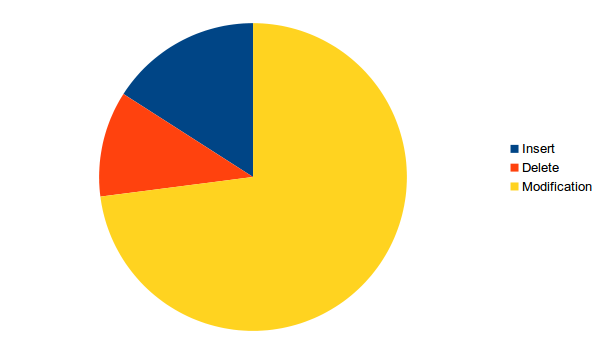
\includegraphics[scale=.8]{TextDifference}
 \end{center}
 \caption{Type of operations for an ordinary text comparision on average for all the benchmarks}
 \label{fig:textDifference}
\end{figure}

When we examine the Java AST differences for the same benchmark however the number of modifications reduces and the number of insertions and deletes increase.
This is shown in Figure \ref{fig:javaDifference}.
The reason for this is because an change done to block of text recorded in the \lstinline{EditList} object is made up of a number of smaller changes.  
If the block of text is a delete all the smaller changes are also delete.  
The same is true for inserts, all the smaller changes will also be inserts.
With a modified block of text modifications however the smaller changes could be inserts, deletes or modifications.
What this means is that some of the changes that an ordinary text diff recognises as modifications could actully made up of individual inserts and deletes. 

\begin{figure}[!t]
 \begin{center}
 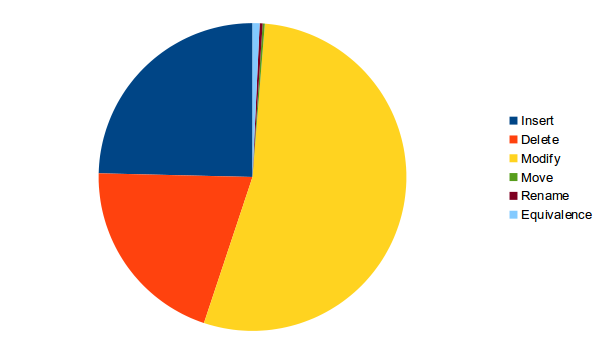
\includegraphics[scale=.8]{JavaDiff}
 \end{center}
 \caption{Type of operations for an ordinary text comparision on average for all the benchmarks}
 \label{fig:javaDifference}
\end{figure}

Most of the changes where still identified as modifications rather than moves, renames or changes to comments. 
There are enough of the changes to comments and moves of the code however to warrent further investigation.

% resons why these benchmarks where used
% 
% 

% There were a number of benchmarks we would have liked to have used but due 
% to memory constraints we had to omit these from the benchmark suite.
% 
% 
% 
%  \begin{table}[H]
%     \small{
%     \begin{tabular}{l|lllll}
%     Benchmark        & Description   & Commits  & LOC   \\ \hline
%     Antlr4             &  \begin{minipage}[t]{0.5\textwidth}
%     A parser generator used to create programming grammers.
% 
% github.com/antlr/antlr4
% \end{minipage}        & 2867      & 40373 \\
% 
%     Clojure             & \begin{minipage}[t]{0.5\textwidth}
%     A programming language that targets the JVM
% github.com/clojure/clojure
% \end{minipage}        & 2602      & 37512   \\
%     gitblit         & \begin{minipage}[t]{0.5\textwidth}
%      Java implementation of Git.
% github.com/gitblit/gitblit
% \end{minipage}       & 2334       & 72188 \\
%     Jacoco            & \begin{minipage}[t]{0.5\textwidth}
%     Library used to determine code coverage.
% github.com/jacoco/jacoco
% \end{minipage}        & 1184     & 25357 \\
%     JGit             & \begin{minipage}[t]{0.5\textwidth}
%     Java implementation of Git developed by the Eclipse Foundation.
% eclipse.org/jgit
% \end{minipage}       & 3285      & 137993  \\
%     Lombok           & \begin{minipage}[t]{0.5\textwidth}
%     A library that used annotaions to extend Java.
% github.com/rzwitserloot/lombok
% \end{minipage}        & 1624      & 39154  \\
%     Revori           & \begin{minipage}[t]{0.5\textwidth}
%     A revision based DBMS.
% github.com/ReadyTalk/revori
% \end{minipage}        & 349      & 18931  \\
%     \end{tabular}
%     }
% \end{table}
% 

% 
% 
% Memory issues
% baselines we could not compare
% the graeter the amount of revisons the more chance that there was a memeory 
% error
% 
% 
% Moves
% Renames
% comment deletion /inserts and modifications
%   the largest change

There were some interesting results for JDiff

% The data sets following are complete git repositories which have been 
% examined to discover the proportion of changes to behaviour compared to 
% ascetic changes that do not affect the behaviour of the program.
% 
% 
% in table ~\ref{tab:DataSets}
% 
% \begin{table}
%   \caption{Complete git repositories that are tested}
%   \label{tab:DataSets}
%   \begin{center}
%     \begin{tabular}{|c|c|c|}
%        Jasm & this a a Java bytecode assembler
%        written for use with the Whiley programming language. & 
% https://github.com/Whiley/Jasm\\
%       foo & bar \\
%     \end{tabular}
%   \end{center}
% \end{table}
% 

% 
% 
% 
% There are a number of Java categories that the Refactor Categories Tool will 
% recognise.  Apart from the traditional insert, delete and modify it will 
% also recognise if an AST Node has been renamed but the content and type of 
% the node remains the same.  It will recognise valid moves within a scope. It 
% will also recognise when the text based merge got it wrong by claiming that 
% the code was not functionally equivalent when in fact it was.
% 
% Apart from this it will also differentiate between Java code and comments.  
% It can tell if comments have been inserted, modified, moved or deleted.  It 
% will also pick up any changes to that white-space that have not already been 
% figured out by the text based comparison.
 
% Comments
%     Insert
%     Delete
%     Modify
%     Move
% White space
%    Modify
% 
% Java
%  Insert
%  Delete
%  Modify
%  Move
%  Rename


% need the results in here
% 
% 
% what this means
% modifications to comments
% 
% modification to comments could be surplus to need
% 
% 
% Examine certain events
% 
% in this case the comment is removed but as the comment is associated with a 
% functional change the comment also needs to change in both versions

